\chapter{Brazo robótico}
\label{ch:BrazoRobotico}

En este capítulo vamos a estudiar el comportamiento y la estructura de un brazo robótico para luego crear un controlador de bajo nivel, un teleoperador, para él. Esta práctica supone la primera incursión en JdeRobot en el ámbito de los brazos robóticos y prepara el terreno para posteriores prácticas de planificación de movimientos articulados con este tipo de robots.

\section{Brazos robóticos existentes en el entorno ROS}
\label{sec:br_brazosexistentes}

Dado que el objetivo no es crear un brazo, sino trabajar sobre uno ya diseñado, comenzamos buscando uno sobre el cual realizar el estudio. Debido a un cambio en la distribución de los paquetes de ROS entre las versiones Indigo y Jade, la mayoría de brazos manipuladores encontrados son antiguos y dan muchos problemas de instalación y configuración en las versiones más modernas. A partir de Indigo, los paquetes que forman ROS Industrial se han separado del núcleo de ROS, no están mantenidos por ROS, por lo que el desarrollo y la corrección de errores es más lenta. Puesto que queremos realizar el trabajo sobre ROS Kinetic y Gazebo 7 necesitamos encontrar un brazo que funcione bajo estas versiones. Tanteamos el uso de varios modelos:
\begin{itemize}
	\item PR2: Se trata de un robot con apariencia de androide (\textit{Figura \ref{fig:pr2}}). Se compone de una base con ruedas, dos brazos y una cabeza con diferentes sensores visuales, siendo los brazos donde centraríamos nuestra atención. Cuando miramos su página de ROS\footnote{\url{http://wiki.ros.org/Robots/PR2}} observamos que no da soporte más allá de Indigo, lo cual puede suponer un problema.
	\begin{figure}[h]
		\centering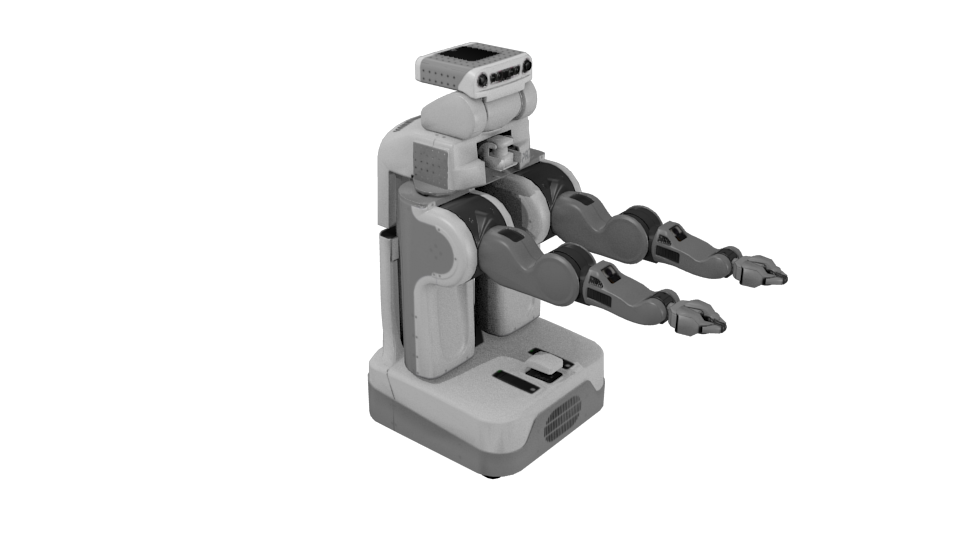
\includegraphics[width=0.95\textwidth]{pr2.png}
		\caption{Robot PR2.}
		\label{fig:pr2}
	\end{figure}
	\item kuka: La empresa Kuka\footnote{\url{https://www.kuka.com/}} fabrica diversos brazos mecánicos y robots industriales. Hay varios modelos disponibles para su uso con Gazebo y ROS, y todos tienen en común el brazo que monta el robot de la Figura \ref{fig:kuka}, aunque la plataforma donde se apoya el brazo puede ser diferente o no estar. En su página de ROS\footnote{\url{http://wiki.ros.org/kuka}} vemos que soporta las versiones de Indigo y Kinetic, pero mediante la instalación del paquete externo ROS-Industrial\footnote{\url{http://wiki.ros.org/Industrial}}.
	\begin{figure}[h]
		\centering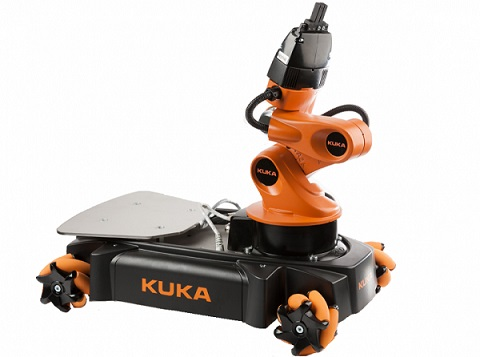
\includegraphics[width=0.50\textwidth]{kuka.jpg}
		\caption{Robot kuka.}
		\label{fig:kuka}
	\end{figure}
	\item ur10: De la empresa Universal Robots\footnote{\url{https://www.universal-robots.com/es/}}. Es un brazo simple (\textit{Figura \ref{fig:ur10}}), al igual que sus hermanos el ur3 y el ur5. La diferencia entre éstos no va más allá del tamaño y fuerza del robot. En su página de ROS\footnote{\url{http://wiki.ros.org/ur_gazebo}} observamos que no da soporte más allá de Indigo, lo cual puede suponer un problema.
	\begin{figure}[h]
		\centering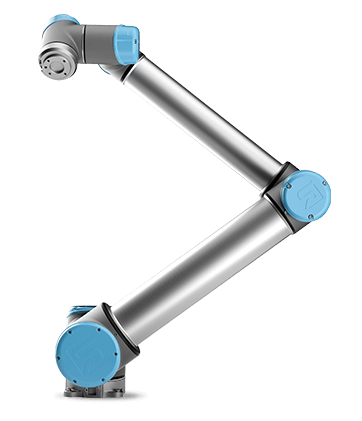
\includegraphics[width=0.45\textwidth]{ur10.png}
		\caption{Robot ur10.}
		\label{fig:ur10}
	\end{figure}
\end{itemize}

Probamos los brazos bajo la última versión de Gazebo y de ROS recurriendo a la extensa comunidad de ROS en busca de soluciones para incorporar los brazos a la última versión. Algunas de las soluciones propuestas y probadas por nosotros son la instalación manual desde fuente, la compilación manual del código fuente, paquetes alternativos de usuarios que han resuelto los problemas de compatibilidad o interfaces de usuarios para que el robot se comunique con las librerías actuales. Después de probar muchas de estas soluciones, y de intentar solucionar los problemas por nuestra cuenta, vemos que ninguno de ellos llega a funcionar de forma correcta bajo nuestros requisitos.

Finalmente recurrimos a los escenarios de ARIAC (\textit{Sección \ref{sec:inf_ariac}}) para desarrollar nuestro trabajo. Como podemos ver en la Figura \ref{fig:ariac01} se trata de un escenario industrial, con un brazo ur10 situado sobre un carril que le permite desplazarse. Nos centramos en esta parte del escenario y del código, estudiando cómo está construido y cómo funciona. Al comprenderlo mejor podemos ver que sigue un esquema como el de la figura \ref{fig:graficobrazo}, similar al de las prácticas de JdeRobot-Academy. Por un lado, está el mundo de Gazebo con todos los componentes del escenario y el brazo. Por otro, el código que desarrollaremos para crear el teleoperador, y entre ellos la interfaz de comunicación de ROS. Las flechas verdes indican los elementos de ROS y de ARIAC que hemos necesitado para comunicarnos con el brazo, y la flecha roja señala la parte creada como consecuencia de este trabajo. Es de gran ayuda para comprender el funcionamiento del mundo y del brazo la página de documentación de ARIAC\cite{ariacwiki} donde se detallan las interfaces de comunicación de los elementos del escenario.

\begin{figure}[h]
	\centering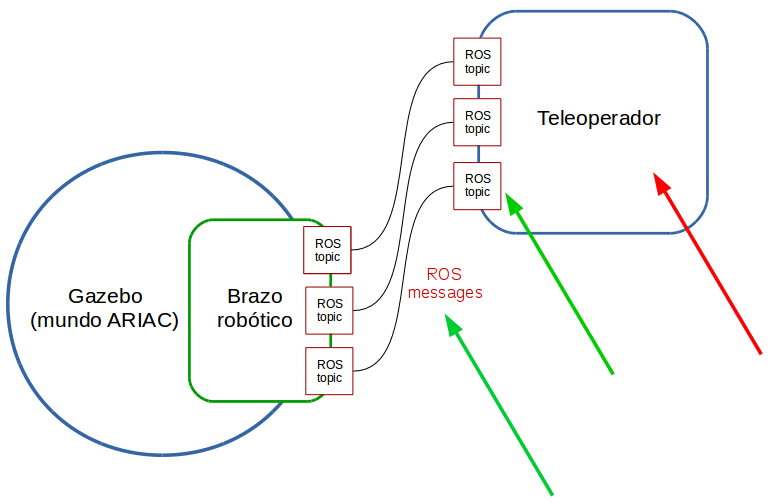
\includegraphics[width=0.7\textwidth]{graficobrazo1.png}
	\caption{Esquema de los componentes de ARIAC centrándonos en el brazo.}
	\label{fig:graficobrazo}
\end{figure}

Para poder avanzar y comenzar a probar cosas sobre el funcionamiento del brazo, necesitamos comprender mejor cómo funciona ROS. 

\section{Hablando ROS con un brazo robótico ARIAC}
\label{sec:br_hablandoros}

\subsection{Nodos y topics}
\label{subsec:br_nodosytopics}

Para aprender el funcionamiento de ROS vamos a la documentación oficial\cite{roswiki}. Una vez allí nos damos cuenta de que los conceptos básicos que conocer para entender ROS son los \textit{topics}, los \textit{nodes} y  los \textit{messages}. 

Los \textit{nodes} son los procesos ejecutables, en nuestro caso escritos en Python, que se combinan entre sí siguiendo un esquema de grafo. Se comunican unos con otros mediante \textit{topics}, servicios y acciones. Está pensado para que cada tarea dentro del robot la ejecute un nodo, facilitando APIs y canales de comunicación que hacen que el conjunto de código sea sencillo de depurar y de utilizar. ROS facilita comandos de terminal como \textit{rosnode list}, que muestra una lista de los nodos activos. Estos comandos son de gran ayuda para entender el funcionamiento del brazo.

Los \textit{topics} son \textit{buses} diferenciables mediante los cuales los nodos intercambian \textit{ROS messages} o mensajes. Normalmente los \textit{topics} y los nodos no se preocupan del destinatario de los mensajes. Los nodos se subscriben a los \textit{topics}, y pueden publicar información en el \textit{topic} haciendo \textit{publish} o recibir información del \textit{topic} haciendo \textit{subscribe}. Por ejemplo un sensor de temperatura o de proximidad publica, mientras que un algoritmo de toma de decisiones o de procesado de datos se subscribe. Son canales de comunicación unidireccionales. Utilizan \textquotedblleft tipado fuerte\textquotedblright  mediante el tipo de \textit{ROS message} que transmiten, de forma que un tipo de mensaje erróneo no se puede transmitir por el \textit{topic} y no producirá fallos en otros nodos. ROS facilita comandos de terminal como \textit{rostopic list} y \textit{rostopic echo /topic\_name}. El primero muestra una lista con los \textit{topics} activos, y el segundo permite ver el flujo de mensajes a través del \textit{topic} deseado. Ambos son una ayuda inestimable para entender, y más tarde replicar, la comunicación con el brazo.

Los \textit{servicios} son canales bidireccionales de comunicación entre nodos. Esto quiere decir que cuando se envía un mensaje, el nodo destino debe enviar otro de respuesta, o la comunicación no tiene éxito. Las \textit{acciones} son un método de comunicación mas directo, como si de una llamada a procedimiento se tratase. Ninguno de estos medios son usados para enviar órdenes al brazo, por lo que no profundizamos en ellos.

Los \textit{ROS messages} contienen la información que los nodos se envían mediante los \textit{topics}. Se trata de estructuras de datos con campos fijos, que soportan tanto tipos de datos primitivos (enteros, \textit{floats}, \textit{boleanos}, etc) como arrays de estos tipos de datos. Estas estructuras están predefinidas en la mayoría de casos comunes, pero se pueden definir nuevas usando archivos en formato .msg donde se especifique la estructura de datos del mensaje

Una vez conocemos los elementos de comunicación probamos cómo se produce, creando un nodo \textit{publisher} y otro \textit{subscriber} y haciendo que hablen entre sí. Mediante los diferentes comandos de terminal que proporciona ROS comprobamos el correcto funcionamiento de los mismos. 

\subsection{Nodos, \textit{topics} y mensajes de un brazo robótico ARIAC}
\label{subsec:br_nododstopicsymensajes}

\begin{figure}[ht]
	\centering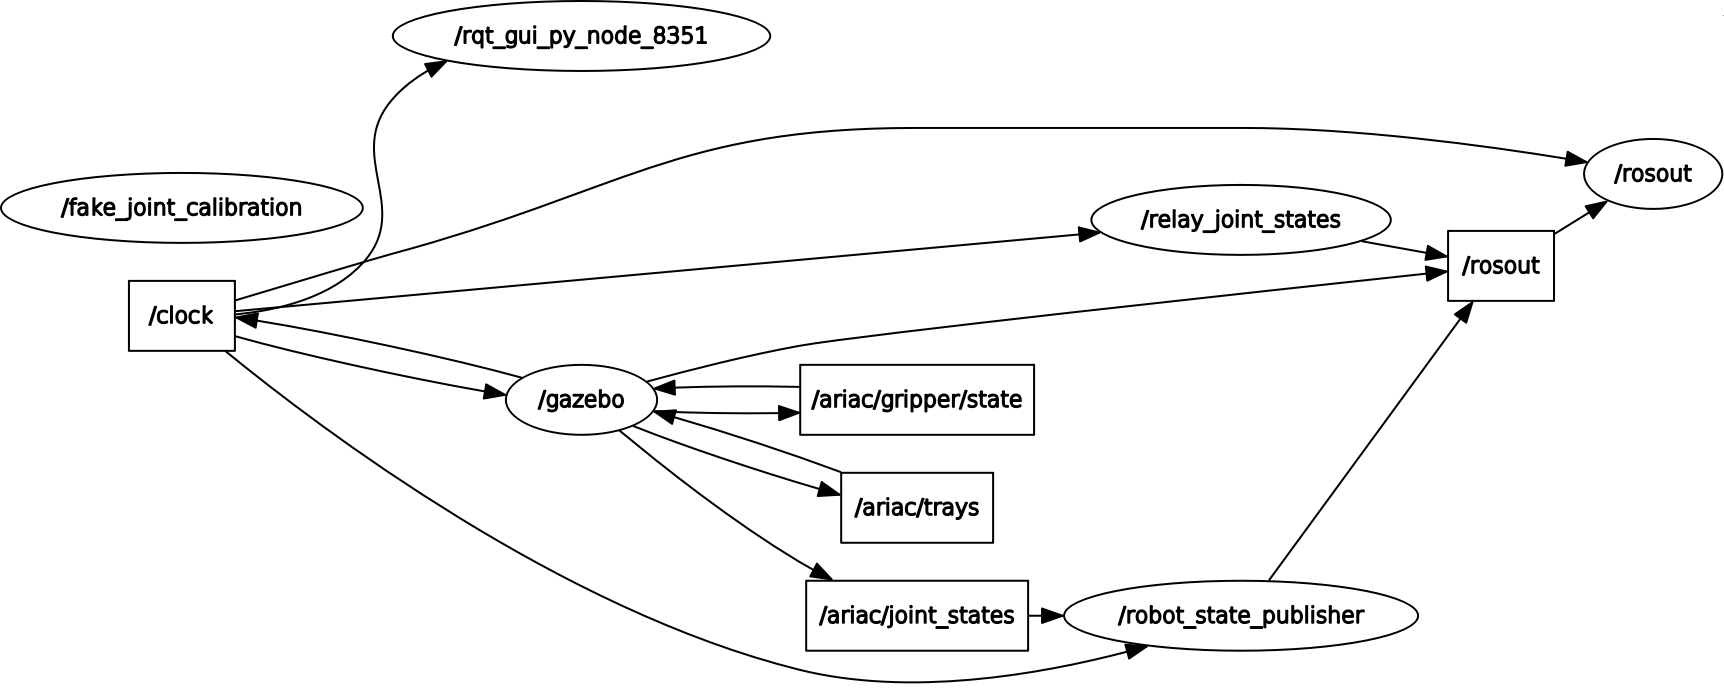
\includegraphics[width=1\textwidth]{Brazo10a.png}
	\caption{Grafo de los \textit{nodes} y \textit{topics} de ARIAC.}
	\label{fig:ariacgraph1}
\end{figure}

Una vez entendemos el funcionamiento de ROS lanzamos el mundo de ARIAC. A través de los comandos visualizamos la lista de nodos y \textit{topics} disponibles. Nos servimos de una herramienta de ROS para obtener un grafo con la relación entre todos ellos y tener una idea clara del funcionamiento y la relación entre los elementos del brazo. Para ellos ejecutamos en la terminal \textit{rosrun rqt\_graph rqt\_graph} y obtenemos la Figura \ref{fig:ariacgraph1}. En dicha figura, los elementos redondos son nodos y los cuadrados son \textit{topics}, y las flechas establecen la relación entre ellos. Si la flecha apunta hacia un \textit{node} desde un \textit{topic} quiere decir que el nodo está subscrito a ese \textit{topic}. Si por el contrario la flecha va desde un \textit{node} a un \textit{topic} quiere decir que el nodo publica en ese \textit{topic}.

\begin{figure}[hb]
	\centering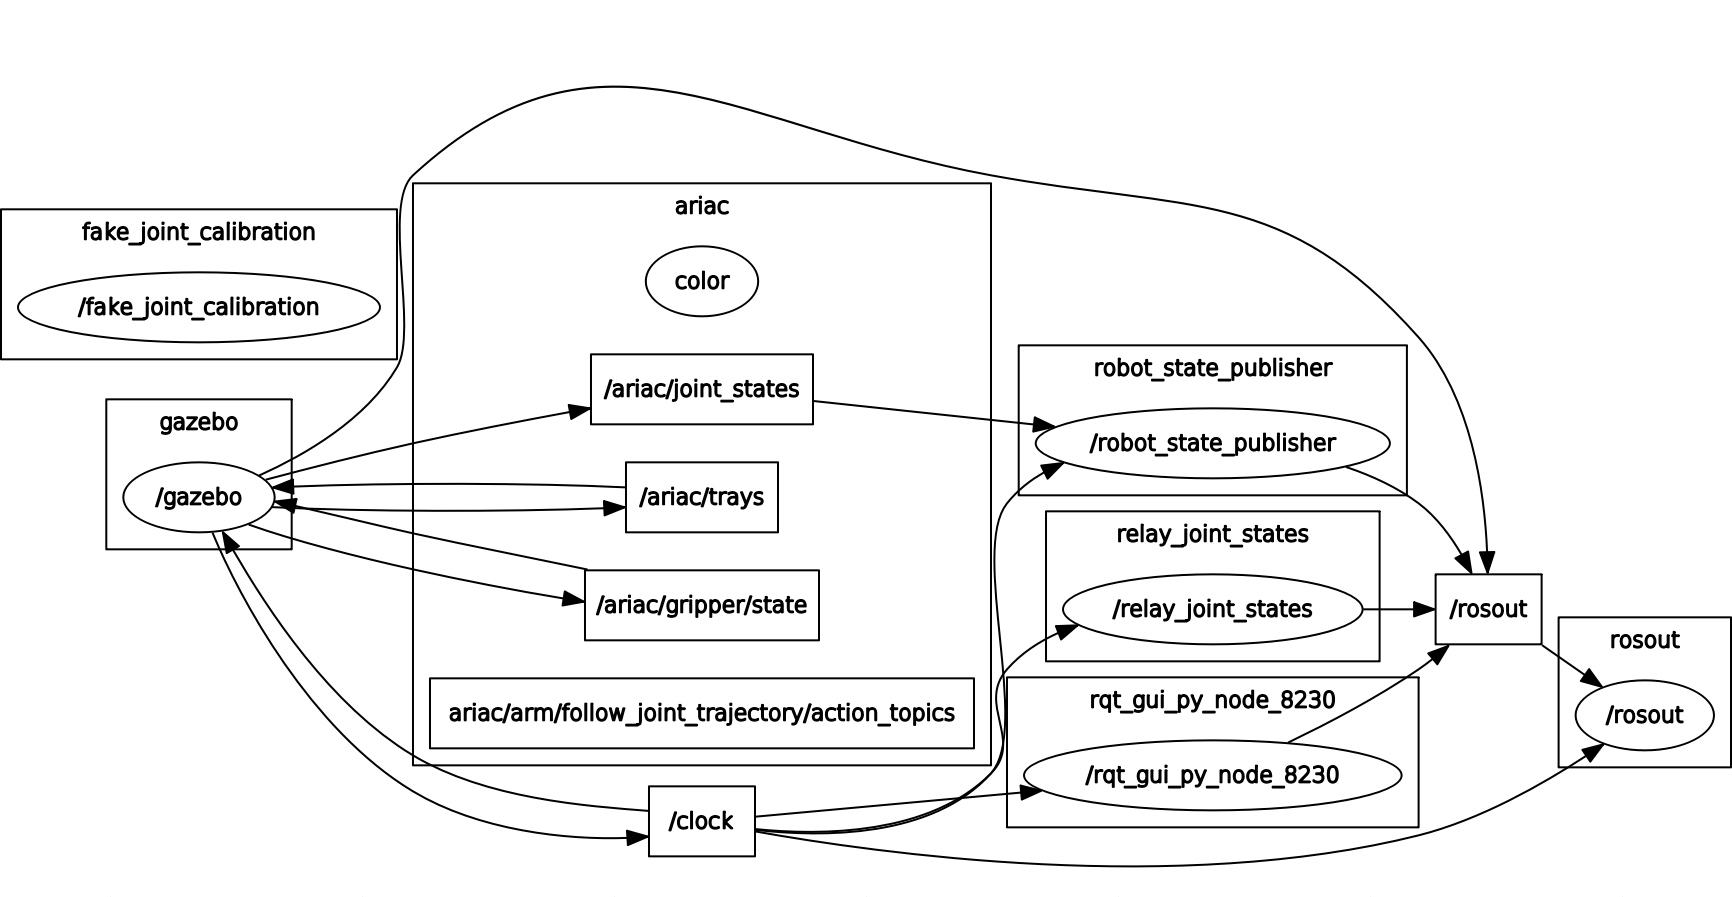
\includegraphics[width=1\textwidth]{Brazo10.png}
	\caption{Grafo de los \textit{nodes} y \textit{topics} de ARIAC.}
	\label{fig:ariacgraph2}
\end{figure}

Aunque ya nos da una idea muy clara de la organización de los nodos y \textit{topics}, la herramienta \textit{rqt\_graph} nos permite agruparlos por nombres. Dado que hay varios \textit{topics} cuyo nombre es “/ariac/nombre”, \textit{rqt} incluye a todos los que tienen ese formato en el nombre en la caja ARIAC. De esta forma la caja ariac hace referencia a todos los nodos y \textit{topics} que comparten el nombre ariac. Si hacemos esto obtenemos el grafo de la figura \ref{fig:ariacgraph2}.

En esa figura podemos diferenciar varios bloques importantes. En el centro del grafo se sitúan los \textit{topics} y nodos referentes al mundo ARIAC, A su izquierda se encuentra el nodo principal de Gazebo. Encima de éste y a la derecha del bloque ariac hay varios grupos que sirven de apoyo para el entorno: \textit{fake\_joint\_calibration}, \textit{robot\_state\_publisher} y \textit{relay\_joint\_states}.
Debajo de ariac se encuentra el topic“/clock”, que sirve de referencia para todos los elementos de la simulación. A la derecha de éste está el nodo de \textit{rqt} que nos permite obtener esta imagen. En la parte derecha del grafo hay diversos nodos y \textit{topics} de \textit{rosout}. Se trata de la consola de \textit{log} de ROS, donde se anotan los sucesos o errores de los diferentes procesos ejecutados.

Una vez tenemos este esquema en la cabeza acudimos tanto al código de ARIAC como a su documentación para ver qué hace cada nodo y cada topic, qué partes controlan el brazo y cómo podemos comunicarnos con ellas. De esta forma descubrimos dos \textit{topics} clave para poder controlar el brazo:
\begin{itemize}
	\item /ariac/joint\_states: En este \textit{topic} se publica la información relativa las posiciones de las articulaciones del brazo. Por este \textit{topic} se envían mensajes de tipo \textit{sensor\_msgs/JointState Message}, que veremos más adelante. Nos subscribiremos a este \textit{topic} para conocer la posición inicial del brazo y de sus articulaciones.
	
	\item /ariac/arm/command: Por este \textit{topic} se envía al brazo la posición a la que quieres moverlo mediante mensajes del tipo \textit{trajectory\_msgs/JointTrajectory Message}, que veremos más adelante. Necesitamos publicar en este \textit{topic} para enviar órdenes al brazo.
	
\end{itemize}

Los demás \textit{topics} tienen otras funciones que no necesitamos para conseguir nuestro objetivo.

Los mensajes descritos anteriormente tienen la siguiente estructura:
\begin{itemize}
	\item \textit{sensor\_msgs/JointState Message}:
	\begin{lstlisting}
	std_msgs/Header header
	string[] name
	float64[] position
	float64[] velocity
	float64[] effort
	\end{lstlisting}
	\item \textit{trajectory\_msgs/JointTrajectory Message}:
	\begin{lstlisting}
	std_msgs/Header header
	string[] joint_names
	trajectory_msgs/JointTrajectoryPoint[] points
	\end{lstlisting}
\end{itemize}

Ambos mensajes comienzan con un \textit{Header} de tipo \textit{std\_msg/Header}. Este es un tipo de mensaje estándar de ROS, que necesitan todos los mensajes para que pueda establecerse la comunicación, y se crea automáticamente al enviar el mensaje. No necesitamos crearlo para poder enviar mensajes y no necesitamos extraerlo al recibirlos, por lo que no nos preocupamos por el.

El primer tipo de mensaje lo componen varios \textit{arrays} de datos primitivos. El primero de ellos es un \textit{array} de \textit{strings}. Los \textit{strings} son cadenas de caracteres, como palabras o frases. Este campo lo componen los nombres de las articulaciones del brazo, que son:
\begin{itemize}
	\item elbow\_joint : Ésta es la articulación del codo, la del medio del brazo.
	
	\item linear\_arm\_actuator\_joint : Ésta no es una articulación propiamente dicha, sino que se refiere a la posición del brazo en el carril sobre el que está situado.
	
	\item shoulder\_lift\_joint : Ésta es la articulación del hombro, es decir, la más cercana a su base. En concreto controla la elevación del brazo. Realiza giros sobre un imaginario eje y.
	
	\item shoulder\_pan\_joint : Ésta es la articulación del hombro, es decir, la más cercana a su base. En concreto controla la orientación del brazo y nos permite girarlo. Realiza giros sobre un imaginario eje z.
	
	\item wrist\_1\_joint : Ésta es la articulación de la muñeca, la más alejada de la base. En concreto controla la elevación de la muñeca y nos permite subirla y bajarla. Realiza giros sobre un imaginario eje y.
	
	\item wrist\_2\_joint : Ésta es la articulación de la muñeca, la más alejada de la base. En concreto controla el giro de la muñeca y nos permite rotarla verticalmente. Realiza giros sobre un imaginario eje z.
	
	\item wrist\_3\_joint : Ésta es la articulación de la muñeca, la más alejada de la base. En concreto controla el giro de la mano y nos permite rotar la muñeca horizontalmente. Realiza giros sobre un imaginario eje x.
	
	\item vacuum\_gripper\_joint : Esta articulación hace referencia a una pinza de vacío que se puede acoplar a la articulación de la muñeca del brazo, pero en nuestro caso no la incorpora y no necesitamos asignarle valores
\end{itemize}

En la Figura \ref{fig:brazoarticulaciones} podemos situar visualmente las articulaciones en el brazo, con la diferencia de que la articulación \textit{Base Joint} de la imagen en ARIAC se llama \textit{shoulder\_pan\_joint}. Todas estas articulaciones tienen definida su posición en radianes y unos límites de giro entre 6,28 y -6,28 en su mayoría. Esto quiere decir que cada articulación del brazo puede realizar dos giros completos si fuese necesario, pero los choques con los elementos de escenario limitan los movimientos.

\begin{figure}[]
	\centering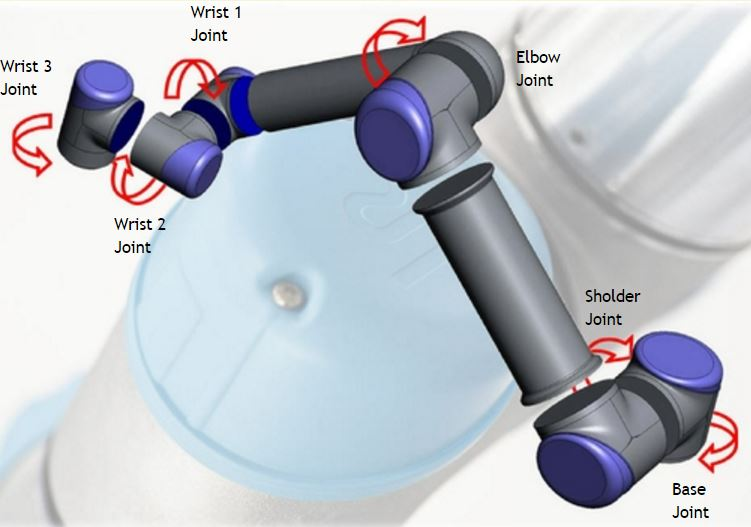
\includegraphics[width=0.7\textwidth]{brazoarticulaciones.jpg}
	\caption{Detalle de las articulaciones del brazo.}
	\label{fig:brazoarticulaciones}
\end{figure}

Los siguientes campos del mensaje son \textit{arrays} de \textit{floats} (números) de posiciones, velocidades y esfuerzos. Dan información de la posición de cada articulación, la velocidad a la que se mueven, y el esfuerzo o fuerza que poseen en el momento de envío del mensaje, por lo que son arrays de ocho posiciones y en cada una está la información relativa a la articulación en la posición homóloga en el array de nombres. A nosotros nos interesa el primer \textit{array} para conocer la posición inicial de las articulaciones.

Para ver mejor la estructura del mensaje lanzamos el mundo de ARIAC y ejecutamos el comando de terminal \textit{rostopic echo /ariac/joint\_states}, obteniendo en texto en la terminal la estructura de datos de este mensaje:
\\
\\
\begin{lstlisting}
---
header: 
seq: 265
stamp: 
secs: 5
nsecs: 322000000
frame_id: ''
name: ['elbow_joint', 'linear_arm_actuator_joint', 'shoulder_lift_joint', 'shoulder_pan_joint', 'wrist_1_joint', 'wrist_2_joint', 'wrist_3_joint', 'vacuum_gripper_joint']
position: [1.5072954794978815, 0.04169673392358113, -0.3793140712872205, 3.217984505432054, 3.085834205511564, -1.6130778569148077, -0.00793595855568796, 0.0]
velocity: [0.027474972846918494, 0.007286219434794008, 0.05461882849916373, 0.0316967471028743, 0.1957558318356749, -1.091011699832568, -8.054309845386587, 0.0]
effort: [150.0, -184.23945050318943, 330.0, 167.6704306272329, 0.0, 5.601291580407757, -5.541011517572109, 0.0]
---
\end{lstlisting}

El \textit{header} o cabecera ocupa las primeras siete líneas, y refleja datos como el tiempo de simulación o el número de mensaje, ninguno de ellos relevante para nosotros. A continuación nos encontramos los cuatro \textit{arrays}: \textit{name} para los nombres de las articulaciones, \textit{position} para las posiciones, \textit{velocity} para las velocidades y \textit{effort} para las fuerzas. Este mensaje es el que recibiremos y que deberemos procesar para obtener la posición inicial del brazo.

El segundo tipo de mensaje lo componen un \textit{array} de \textit{strings} y otro campo llamado \textit{points} compuesto por otro tipo de mensaje, el tipo \textit{trajectory\_msgs/JointTrajectoryPoint}. El primer \textit{array} hace referencia a los nombres de las articulaciones, pero en este mensaje se llama \textit{joint\_names} Como podemos ver a continuación, este tipo de mensaje está formado por \textit{arrays} de números de forma muy similar a los del primer mensaje:
\begin{lstlisting}
float64[] positions
float64[] velocities
float64[] accelerations
float64[] effort
duration time_from_start
\end{lstlisting}
Tenemos un \textit{array} para las posiciones, otro para las velocidades, otro para las aceleraciones, otro para las fuerzas, y un último campo de tipo \textit{duration} para especificar el número de segundos desde el inicio para ejecutar los movimientos. Nosotros usaremos tanto el \textit{array} de nombres como el de posiciones, así como el campo para establecer el tiempo inicial de la orden. Los demás campos no son necesarios para el correcto funcionamiento del brazo.

De la misma forma que con el mensaje anterior, arrancamos la simulación y ejecutamos en la terminal el comando \textit{rostopic echo /ariac/arm/commander} para obtener en texto el contenido de los mensajes que pasan por este \textit{topic}. Nos servimos de los tutoriales para dar órdenes sencillas a través de comandos de terminal y poder capturar el contenido de estos mensajes:
\begin{lstlisting}
---
header: 
seq: 59
stamp: 
secs: 0
nsecs:         0
frame_id: ''
joint_names: ['elbow_joint', 'linear_arm_actuator_joint', 'shoulder_lift_joint', 'shoulder_pan_joint', 'wrist_1_joint', 'wrist_2_joint', 'wrist_3_joint']
points: 
- 
positions: [1.510634135925831, 1.4199980429372933e-06, -1.1286545928274752, 3.140002031709801, 3.772089274964015, -1.5100101552695162, 4.0770707014914365e-06, 0.0]
velocities: []
accelerations: []
effort: []
time_from_start: 
secs: 1
nsecs:         0
---
\end{lstlisting}
Al igual que en el primer tipo de mensaje, la cabecera la componen las siete primeras líneas. Después nos encontramos con el \textit{array} de nombres de articulaciones. A continuación nos encontramos con el campo \textit{points}, es decir, el campo que contiene otro tipo de mensaje. Dentro podemos ver los cuatro arrays, y comprobamos que sólo el de posiciones está definido, los demás están en blanco y no son imprescindibles para dar órdenes al brazo. Por último podemos ver el campo \textit{time\_from\_start}, el cual establece el tiempo en 1 segundo.


\section{Teleoperador de un brazo robotizado}
\label{sec:br_teleoperador}

Una vez estudiados los mensajes y los \textit{topics} que necesitamos para controlar el brazo comenzamos a implementar el controlador. Utilizando Python como lenguaje, creamos un archivo en el que vamos probando paso a paso la aplicación de los conceptos adquiridos, tanto de ROS como de ARIAC. 
Primero creamos un nodo al que llamaremos “Mando”. Luego hacemos que se subscriba al \textit{topic} \textit{/ariac/joint\_states}, que descomponga los mensajes recibidos y que imprima por terminal los datos extraídos. 

A continuación hacemos que el nodo publique en el \textit{topic /ariac/arm/command} una orden predefinida que hace que se mueva ligeramente, simplemente para comprobar que el envío de un mensaje bien construido a este \textit{topic} consigue mover el brazo. Para ello debemos construir el mensaje de acuerdo a las especificaciones anteriormente descritas. Vemos que es necesario introducir el envío de mensajes en un bucle, ya que si enviamos uno y salimos, ROS cierra el nodo antes de que el mensaje llegue, con lo que no se recibe.

Una vez realizadas estas tareas pasamos a desarrollar la interfaz gráfica que nos permita controlar el brazo visualmente. Nos servimos de Qt para desarrollar la interfaz visual. Creamos unos deslizadores para cambiar los valores de posición de cada articulación por separado, consiguiendo de una forma heurística saber dónde están los límites de cada articulación y cuál es su posición respecto al total de su movimiento. También creamos unas etiquetas que muestran el valor numérico de la posición del deslizador, así como unas etiquetas con el nombre de la articulación que controla cada uno. 

\begin{figure}[]
	\centering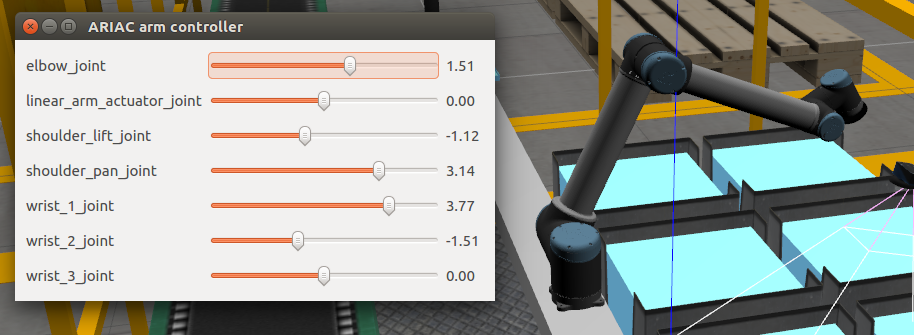
\includegraphics[width=0.9\textwidth]{mando.png}
	\caption{Interfaz gráfica del controlador del brazo y brazo en la posición inicial.}
	\label{fig:mando}
\end{figure}

En lugar de utilizar la interfaz gráfica proporcionada por Qt para construir nuestra GUI la escribimos directamente en código utilizando las propiedades de auto-colocación de objetos. Qt nos permite insertar los elementos como si de una tabla se tratase y automáticamente los separa y les da un espacio suficiente para mostrarse completos. También resulta más fácil programar después el comportamiento de la interfaz, ya que tenemos un mayor control sobre lo que creamos. 

A la hora de crear el controlador agrupando todos los elementos, podemos organizar el código en base a si es relativo a la interfaz o a ROS, por lo que lo dividimos en dos carpetas dentro de la carpeta principal: \textit{gui} y \textit{ros\_manager}. Organizamos todo el código necesario en cinco ficheros:
\begin{itemize}
	\item \textit{main.py}: Este fichero es el encargado de lanzar los procesos relativos a la interfaz y a ROS. Es, por tanto, el ejecutable que invocamos para abrir el controlador. Se encuentra en la carpeta principal, y lanza los hilos de ejecución tanto de ROS como de la interfaz. Las partes más importantes del código de este fichero son:
	\lstset{language=Python}
	\begin{lstlisting}
	ros_manager = RosManager()
	(...)
	myGUI = Window(ros_manager)
	(...)
	t = ThreadGUI(myGUI)
	(...)
	t.start()
	\end{lstlisting}
	
	En la primera línea creamos el objeto que contiene las funciones que se comunican con ROS. En la línea 3 y 5 inicializamos la ventana y el hilo donde se va a ejecutar, finalmente en la línea 7 arrancamos el hilo que gestiona la ventana gráfica. 
	
	\item \textit{gui.py}: En este fichero se encuentran definidos los elementos de la interfaz gráfica, así como el comportamiento de los mismos. Aquí creamos cada elemento, lo colocamos en la ventana, definimos los \textit{callbacks} de los deslizadores y capturamos el cierre de la ventana para realizar un cierre ordenado. Los \textit{callbacks} nos permiten capturar el movimiento de cada deslizador, actualizar la etiqueta correspondiente y enviar el nuevo valor al brazo. El cierre ordenado es necesario para poder cerrar el nodo de ROS y no dejar elementos corriendo en el sistema. A continuación se muestra parte del código utilizado, resumiendo aquellas partes repetitivas donde se repite la misma acción para varios elementos.
	
	Creamos el objeto de Qt que creará el espacio para desplegar los elementos de la ventana:
	\begin{lstlisting}
	mainLayout = QGridLayout()
	\end{lstlisting}
	
	Creamos las etiquetas de cada articulación y escribimos el texto que aparecerá en la ventana, en este caso el nombre real de cada articulación:
	\begin{lstlisting}
	self.label1 = QLabel("elbow_joint")
	(...)
	self.label7 = QLabel("wrist_3_joint")
	\end{lstlisting}
	
	Creamos los deslizadores y asignamos los valores límite a cada uno. Como valor inicial preguntamos, a través de \textit{ros\_manager}, la posición real de esa articulación y la redondeamos a dos decimales. En el caso de los deslizadores tiene truco, ya que no saben trabajar con valores decimales. Por eso, aunque los valores mostrados son los reales, trabajamos con ellos con los valores multiplicados por cien, de forma que manejan con números enteros:
	\begin{lstlisting}
	self.slider1 = QSlider(Qt.Horizontal)
	self.slider1.setMinimum(-628)
	self.slider1.setMaximum(628)
	self.slider1.setValue(float('%.2f'%(self.ros_manager.read_elbow()))*100)
	(...)
	self.slider7 = QSlider(Qt.Horizontal)
	self.slider7.setMinimum(-628)
	self.slider7.setMaximum(628)
	self.slider7.setValue(float('%.2f'%(self.ros_manager.read_wrist_3()))*100)
	\end{lstlisting}
	
	Creamos las etiquetas que muestran los valores de las articulaciones y, al igual que con los deslizadores, les damos el valor inicial real del brazo:
	\begin{lstlisting}
	self.value1 = QLabel('%.2f'%(self.ros_manager.read_elbow()))
	(...)
	self.value7 = QLabel('%.2f'%(self.ros_manager.read_wrist_3()))
	\end{lstlisting}
	
	Añadimos uno a uno todos los elementos creados, tanto las etiquetas de los nombres como los deslizadores como las etiquetas de los valores, al elemento de Qt que los mostrará por pantalla. También les damos una ubicación mediante unas coordenadas. las coordenadas (0,0) corresponden a la primera posición, arriba a la izquierda. La posición (1,0) está situada debajo de la primera, mientras que la (0,1) está a la derecha, y así hasta el tamaño deseado. En nuestra ventana el último elemento se coloca en la posición (6,2):
	\begin{lstlisting}
	mainLayout.addWidget(self.label1,0,0)
	(...)
	mainLayout.addWidget(self.label7,6,0)
	mainLayout.addWidget(self.slider1,0,1)
	(...)
	mainLayout.addWidget(self.slider7,6,1)
	mainLayout.addWidget(self.value1,0,2)
	(...)
	mainLayout.addWidget(self.value7,6,2)
	\end{lstlisting}
	
	Definimos la conexión de los \textit{callbacks} entre cada deslizador y la función que procesará el movimiento de este:
	\begin{lstlisting}
	self.slider1.valueChanged.connect(self.valuechange1)
	(...)
	self.slider7.valueChanged.connect(self.valuechange7)
	\end{lstlisting}
	
	Como ya hemos posicionado todos los elementos, damos la orden para que cree la ventana y coloque los elementos en el sitio que hemos asignado. Definimos un nombre para que lo muestre en la barra de título:
	\begin{lstlisting}
	self.setLayout(mainLayout)
	self.setWindowTitle("ARIAC arm controller")
	\end{lstlisting}
	
	Aquí se muestra una de las funciones a las que enlazan los \textit{callbacks}. Lo que hace es coger el valor a donde hemos movido el deslizador, enviarlo (a través de \textit{ros\_manager}) al brazo para que se mueva a esa posición, y cambiar la etiqueta de la ventana con el nuevo valor:
	\begin{lstlisting}
	def valuechange1(self):
	num = self.slider1.value()
	self.ros_manager.move_elbow(float(num)/100)
	self.value1.setText(str(float(num)/100))
	\end{lstlisting}
	
	Con esta función controlamos el cierre. Al intentar cerrar la ventana, esta función pausa el cierre y manda la orden de parada al componente de comunicación con ROS para que pueda salir ordenadamente, y continúa con el cierre:
	\begin{lstlisting}	
	def closeEvent(self, event):
	self.ros_manager.stop()
	event.accept()
	\end{lstlisting}

	\item \textit{threadGUI.py}: Este fichero crea un hilo de ejecución para los elementos de la interfaz gráfica. Dado que este elemento es común a todas las ventanas creadas con Qt, usamos el proporcionado en los tutoriales. Básicamente es un bucle en el que cada cierto tiempo actualiza todos los elementos de la ventana con los valores que hayan cambiado. 
	
	\item \textit{ros.py}: En este fichero se encuentra el código relativo a ROS, el que gestiona el envío y recepción de mensajes. Aquí creamos el nodo, nos subscribimos al brazo, publicamos en él, gestionamos los cambios de posición de los deslizadores de la ventana y controlamos el cierre ordenado del nodo ROS. A continuación mostramos parte del código, resumiendo las partes repetitivas.
	
	Con esta función se crean los parámetros iniciales del objeto que se comunicará con ROS. Primero se conecta con el topic de ROS donde publicará los mensajes para mover el brazo. Define el array con los nombres de las articulaciones y con las posiciones que enviará en los mensajes. Este array de posiciones es muy importante, ya que en él se escriben los valores de posición cada vez que se mueve un deslizador en la ventana, y de aquí se recogen cada vez que se envían al brazo. Después crea un \textit{lock} o candado para evitar errores de concurrencia. Al haber varios hilos en ejecución, se puede dar el caso de que una función quiera escribir en un dato al mismo tiempo que otra quiere cogerlo, produciendo un error. Al “dar” el candado a una sola función, sólo esa puede tocar ese dato, las demás deben esperar a que acabe, evitando estos errores. Por último, llama a la función \textit{start}:
	\begin{lstlisting}
	def __init__(self):
		self.pub = rospy.Publisher("/ariac/arm/command", JointTrajectory, queue_size=10)
		
		self.arm_joint_names = [
			'elbow_joint',
			'linear_arm_actuator_joint',
			'shoulder_lift_joint',
			'shoulder_pan_joint',
			'wrist_1_joint',
			'wrist_2_joint',
			'wrist_3_joint',
			]
			
		self.position = [0.00, 0.00, 0.00, 0.00, 0.00, 0.00, 0.00, 0.00]
		
		self.lock = threading.Lock()
		(...)
		self.start()
	\end{lstlisting}
	
	Esta es la función que se llama cuando se crea el objeto. Lo primero que hace es crear un nodo ROS. Después se subscribe al nodo que publica la información de los estados del brazo, recibe un mensaje y se lo pasa a la función \textit{get\_msg} que interpreta la información contenida en él. Por último, arranca el hilo de ejecución que nos permitirá comunicarnos con el brazo:
	\begin{lstlisting}
	def start(self):
		rospy.init_node('Mando', anonymous=True)

		sub = rospy.Subscriber("/ariac/joint_states", JointState, self.get_msg)
		(...)
	
		self.thread.start()
	\end{lstlisting}
	
	Esta función se llama al recibir el primer mensaje, y obtiene la posición de cada articulación y la almacena para poder inicializar los valores de la ventana. Podemos ver cómo antes de escribir los valores “coge” el candado y después lo “suelta”:
	\begin{lstlisting}
	def get_msg(self, msg):
		self.lock.acquire()
		self.position[0] = msg.position[0]
		(...)
		self.position[7] = msg.position[7]
		self.lock.release()
	\end{lstlisting}
	
	Esta función se usa para enviar mensajes al brazo. Primero construye el mensaje según la estructura de arrays vista anteriormente en este mismo capítulo, y una vez construido lo publica en el \textit{topic} al que se ha subscrito:
	\begin{lstlisting}
	def send_msg(self):
		msg = JointTrajectory()
		msg.joint_names = self.arm_joint_names
		point = JointTrajectoryPoint()
		self.lock.acquire()
		point.positions = self.position
		self.lock.release()
		point.time_from_start = rospy.Duration(1.0)
		msg.points = [point]
		if not rospy.is_shutdown():
			self.pub.publish(msg)
	\end{lstlisting}
	
	La siguiente función es la responsable de que al mover un deslizador en la ventana se pueda enviar ese valor al brazo. Aunque sólo se muestra la de una articulación, las demás siguen el mismo esquema. Simplemente escribe el nuevo valor en el array de posiciones y llama a la función que envía el mensaje:
	\begin{lstlisting}
	def move_elbow(self, pos):
		self.lock.acquire()
		self.position[0] = pos
		self.lock.release()
		self.send_msg()
	\end{lstlisting}
	
	La siguiente función, al contrario de la anterior, contesta a las peticiones de los elementos de la ventana con el valor de la posición pedida. Al igual que la anterior, sólo se muestra una ya que las demás son muy similares:
	\begin{lstlisting}
	def read_elbow(self):
		self.lock.acquire()
		a = self.position[0]
		self.lock.release()
		return a
	\end{lstlisting}

	La última función es la encargada de realizar el cierre ordenado de los elementos de ROS. Además de imprimir un mensaje informando de que se ha iniciado la secuencia de cierre, apaga el nodo de ROS, ya que de no hacerlo se quedaría arrancado pero sin hacer nada hasta que se cierre el proceso principal de ROS:
	\begin{lstlisting}
	def stop(self):
		print("Exiting the ARIAC arm controller... \n")
		(...)
		self.pub.unregister()
		rospy.signal_shutdown("Node Closed")
	\end{lstlisting}	
	
	\item \textit{threadPublisher.py}: Este fichero crea un hilo de ejecución para los elementos de ROS. Dado que no es nuevo ni único para nuestro proyecto, reutilizamos uno de los usados en otros controladores de JdeRobot, simplemente cambiando el objeto de control del hilo. El funcionamiento básico de este hilo es crear un bucle en el que cada cierto tiempo se le envía al brazo un mensaje con la orden de movimiento. Aunque parezca extraño estar constantemente enviando mensajes, es la forma oficial, tanto en los tutoriales como en los ejemplos de la página de ROS, de comunicarse con los actuadores de los robots.

\end{itemize}

\begin{figure}[]
	\centering
	\subfigure[elbow\_joint.]{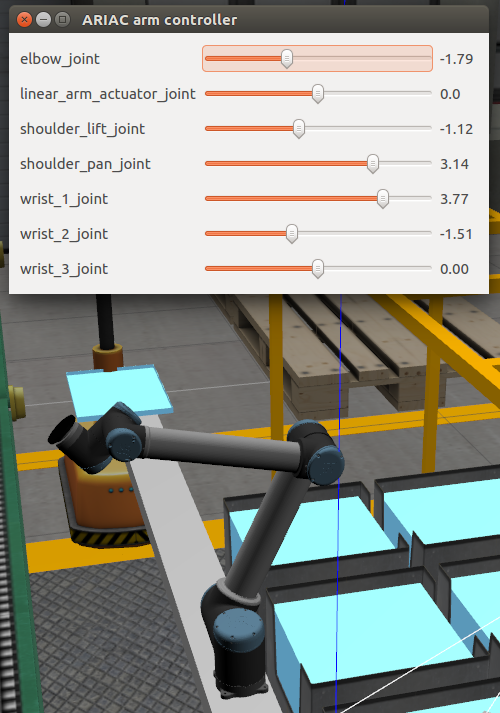
\includegraphics[width=0.445\textwidth]{brazopos1.png}}\hspace{0.07\textwidth}	
	\subfigure[linear\_arm\_actuator\_joint.]{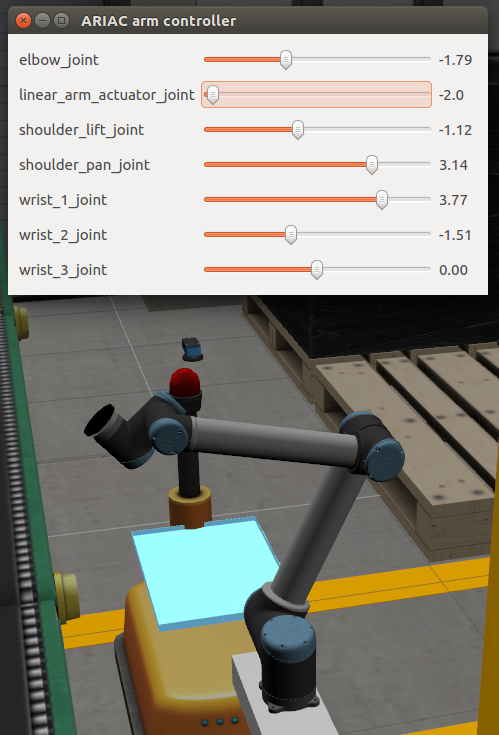
\includegraphics[width=0.433\textwidth]{brazopos2.png}}
	\subfigure[shoulder\_lift\_joint.]{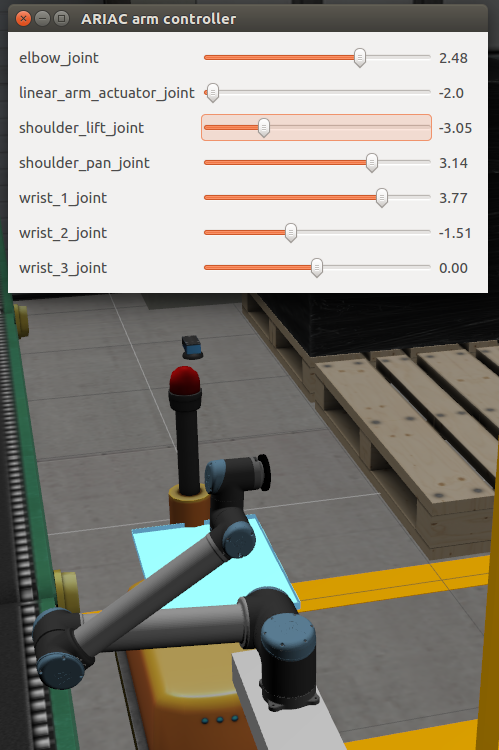
\includegraphics[width=0.434\textwidth]{brazopos3.png}}\hspace{0.07\textwidth}
	\subfigure[shoulder\_pan\_joint.]{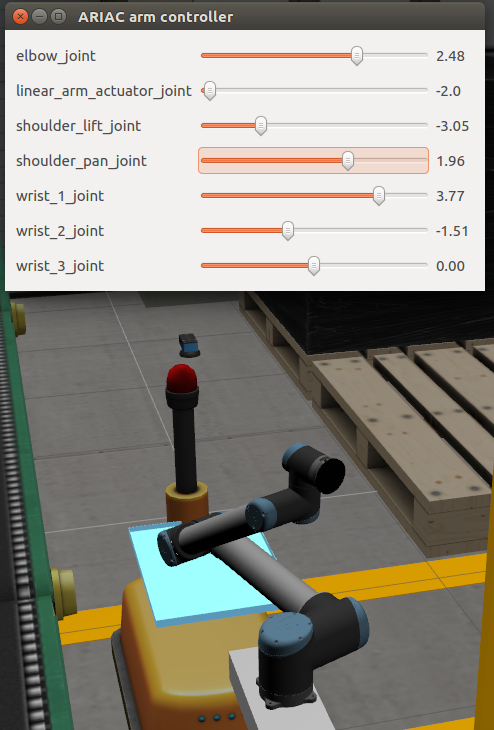
\includegraphics[width=0.44\textwidth]{brazopos4.png}}
	\caption[Ilustración de los grados de libertad del brazo.]{Posiciones de las articulaciones del brazo después de: mover el codo (a); desplazarlo en el carril (b); mover el hombro (c); girar el hombro (d).} \label{fig:posicionesbrazo1}
\end{figure}

\begin{figure}[]
	\centering
	\subfigure[wrist\_1\_joint.]{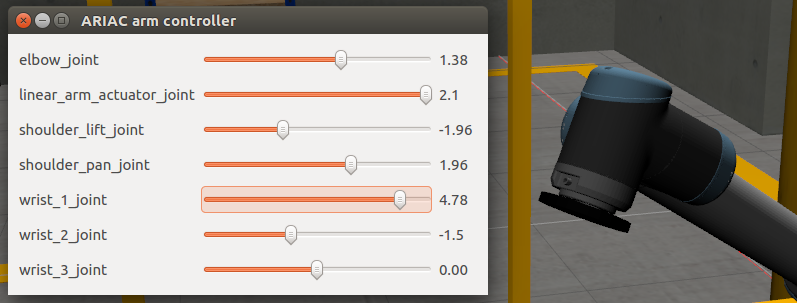
\includegraphics[width=0.85\textwidth]{brazopos5.png}}
	\subfigure[wrist\_2\_joint.]{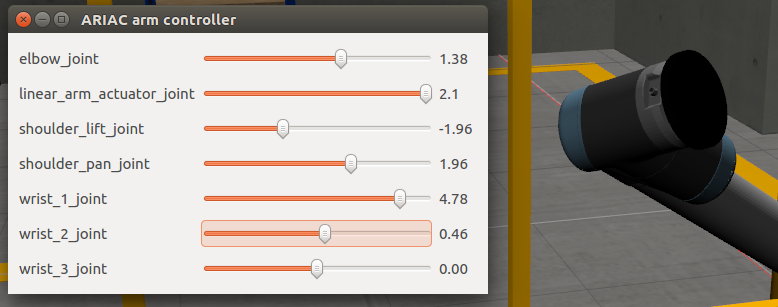
\includegraphics[width=0.85\textwidth]{brazopos6.png}}
	\subfigure[wrist\_3\_joint.]{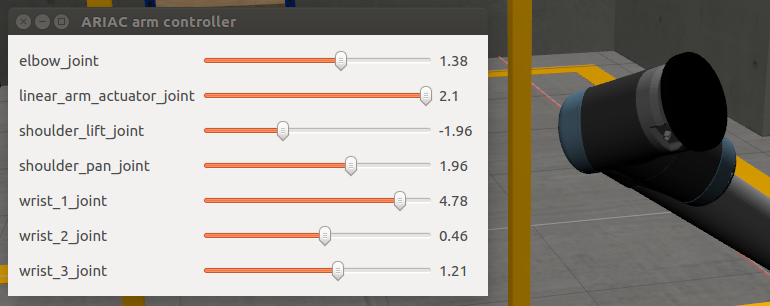
\includegraphics[width=0.85\textwidth]{brazopos7.png}}
	\caption[Ilustración de los grados de libertad de la muñeca.]{Posiciones de las articulaciones de la muñeca después de: girarla en vertical (a); girarla en horizontal (b); girar la mano (c).} \label{fig:posicionesbrazo2}
\end{figure}

En la Figura \ref{fig:mando} podemos ver la apariencia final del controlador del brazo con el que completamos nuestro objetivo inicial, así como la posción inicial del brazo al cargar el mundo de ARIAC. 

Para ilustrar mejor los movimientos del brazo hemos realizado capturas de pantalla en las que se ilustran los grados de libertad del brazo. Se puede ver también el teleoperador, con el deslizador responsable del movimiento de la articulación resaltado. Si nos fijamos en el valor del deslizador que controla esa articulación veremos que es diferente, y se corresponde con la posición del brazo de la imagen. Dado que son siete grados de libertad en total, los hemos repartido en dos figuras. 

En la figura \ref{fig:posicionesbrazo1} podemos ver los movimientos de las articulaciones del brazo, sin la muñeca, partiendo de la posición inicial de la figura \ref{fig:mando}. El na primera imagen mostramos el movimiento del codo. En la segunda desplazamos el brazo hasta el final del carril. En la tercera movemos el hombro, y recolocamos el codo para no colisionar con otros elementos del escenario. En la última giramos el hombro.

En la figura \ref{fig:posicionesbrazo2} podemos ver los movimientos de las articulaciones de la muñeca. En la primera imagen vemos como se ha inclinado hacia delante al mover la primera articulación. Al mover la segunda conseguimos girarla, como muestra la segunda imagen. En la tercera giramos la mano. Se puede apreciar por la muesca lateral que tiene el brazo cerca del disco de su extremo, que de la segunda a la tercera imagen se desplaza debido a este giro.

\section{Manejo del brazo a través del planificador MoveIt}
\label{sec:br_moveit}

Al indagar y realizar pruebas sobre el funcionamiento de ARIAC y de ROS, vemos que existen herramientas que facilitan el control del brazo planificando movimientos. Una de ellas es MoveIt!, que se encarga de calcular trayectorias para facilitar los movimientos, lo que podríamos llamar un controlador de alto nivel. Esto lo hace conociendo el punto de partida del robot y recibiendo el punto de destino o un conjunto de puntos que le sirven de puntos de ruta a través de los cuales calcula la trayectoria. Es una herramienta compleja, ya que debe coordinar todas las articulaciones para que se desplacen hasta el punto final de una forma eficiente y sin chocar entre si. 

\begin{figure}[h]
	\centering
	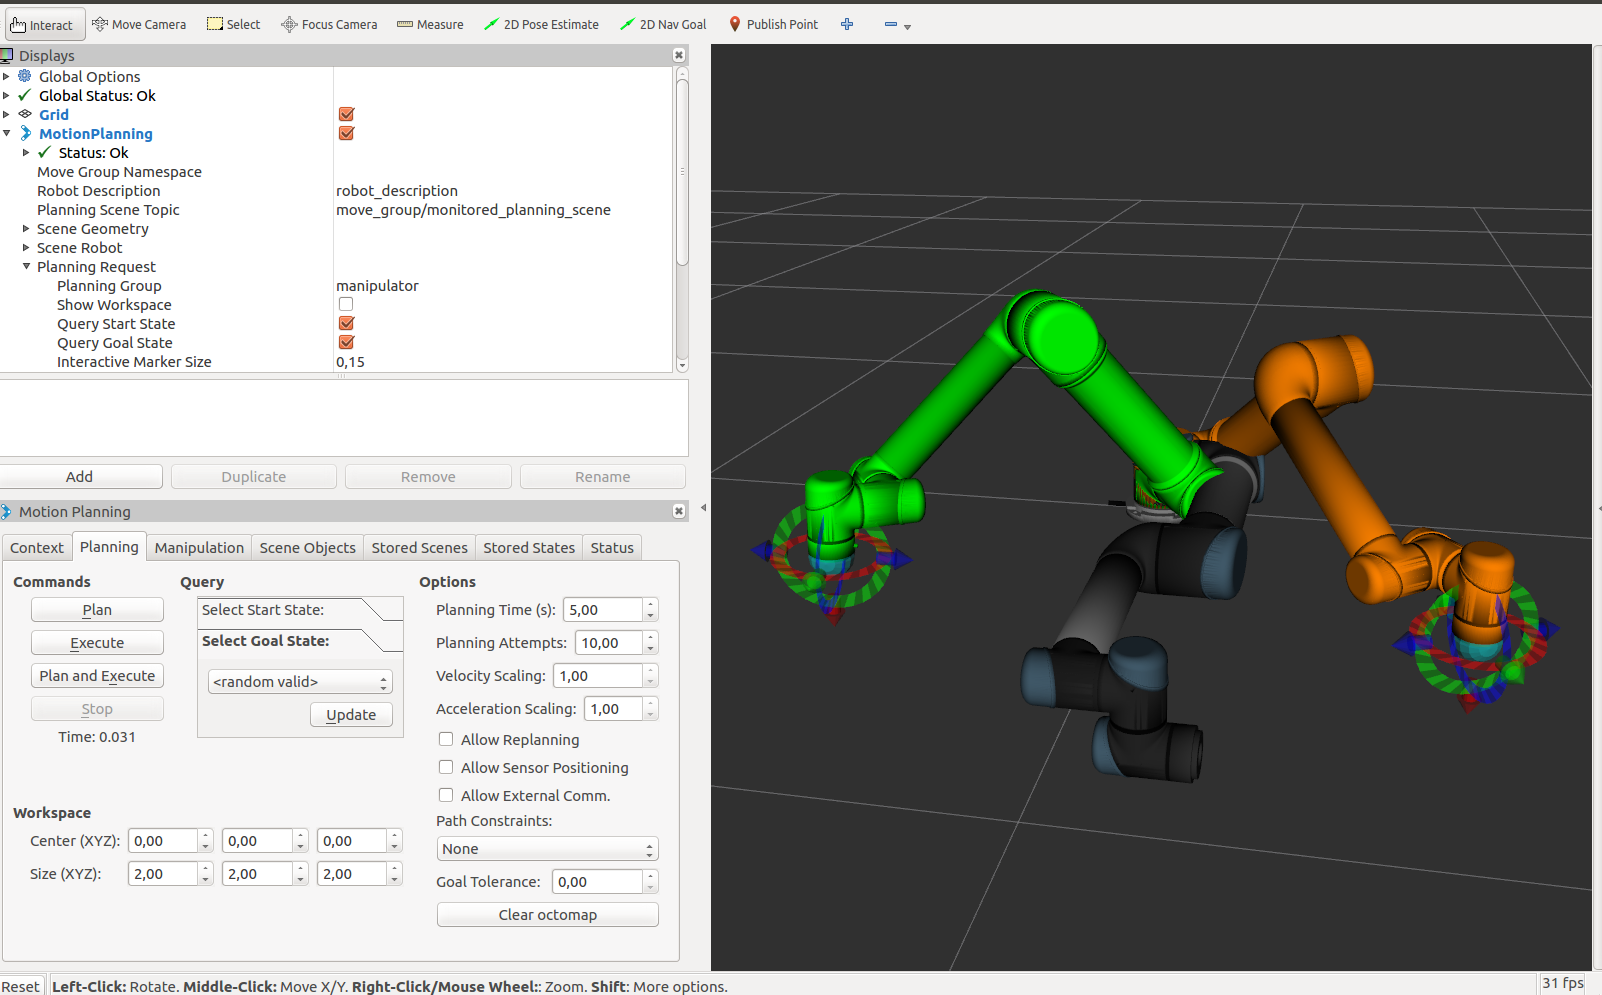
\includegraphics[width=1\textwidth]{Brazo04.png}
	\caption{Herramienta rViz mostrando la trayectoria del brazo.} \label{fig:rviz}
\end{figure}

Se sirve de herramientas como rViz para visualizar el robot, el punto de destino y la trayectoria, como podemos ver en la figura \ref{fig:rviz}. En esta imagen podemos ver el brazo en su posición actual, al igual que se encuentra en Gazebo, y dos siluetas, una verde y otra naranja. La silueta verde identifica la posición de inicio, mientras que la naranja la posición final. En la “mano” del robot podemos ver una bola rodeada de flechas y circunferencias de colores. Esa bola es el punto de referencia que MoveIt utiliza para calcular la trayectoria. Simplemente movemos esa bola por el espacio y la silueta se moverá para posicionar el brazo de forma que la bola esté donde nosotros queremos. Las flechas y círculos de colores son ayudas para mover y rotar la bola en torno a los ejes cartesianos. 

Una vez alcanzada la posición final que queremos, MoveIt podrá planificar (y ejecutar si así lo deseamos) los movimientos necesarios para que el brazo alcance esa posición, sin que tengamos que preocuparnos por nada más.

Para conocer mejor el funcionamiento de esta herramienta utilizamos \textit{rqt} al igual que hicimos para estudiar el funcionamiento de ARIAC, y obtenemos el grafo de la figura \ref{fig:moveitgraph1}.

\begin{figure}[h]
	\centering
	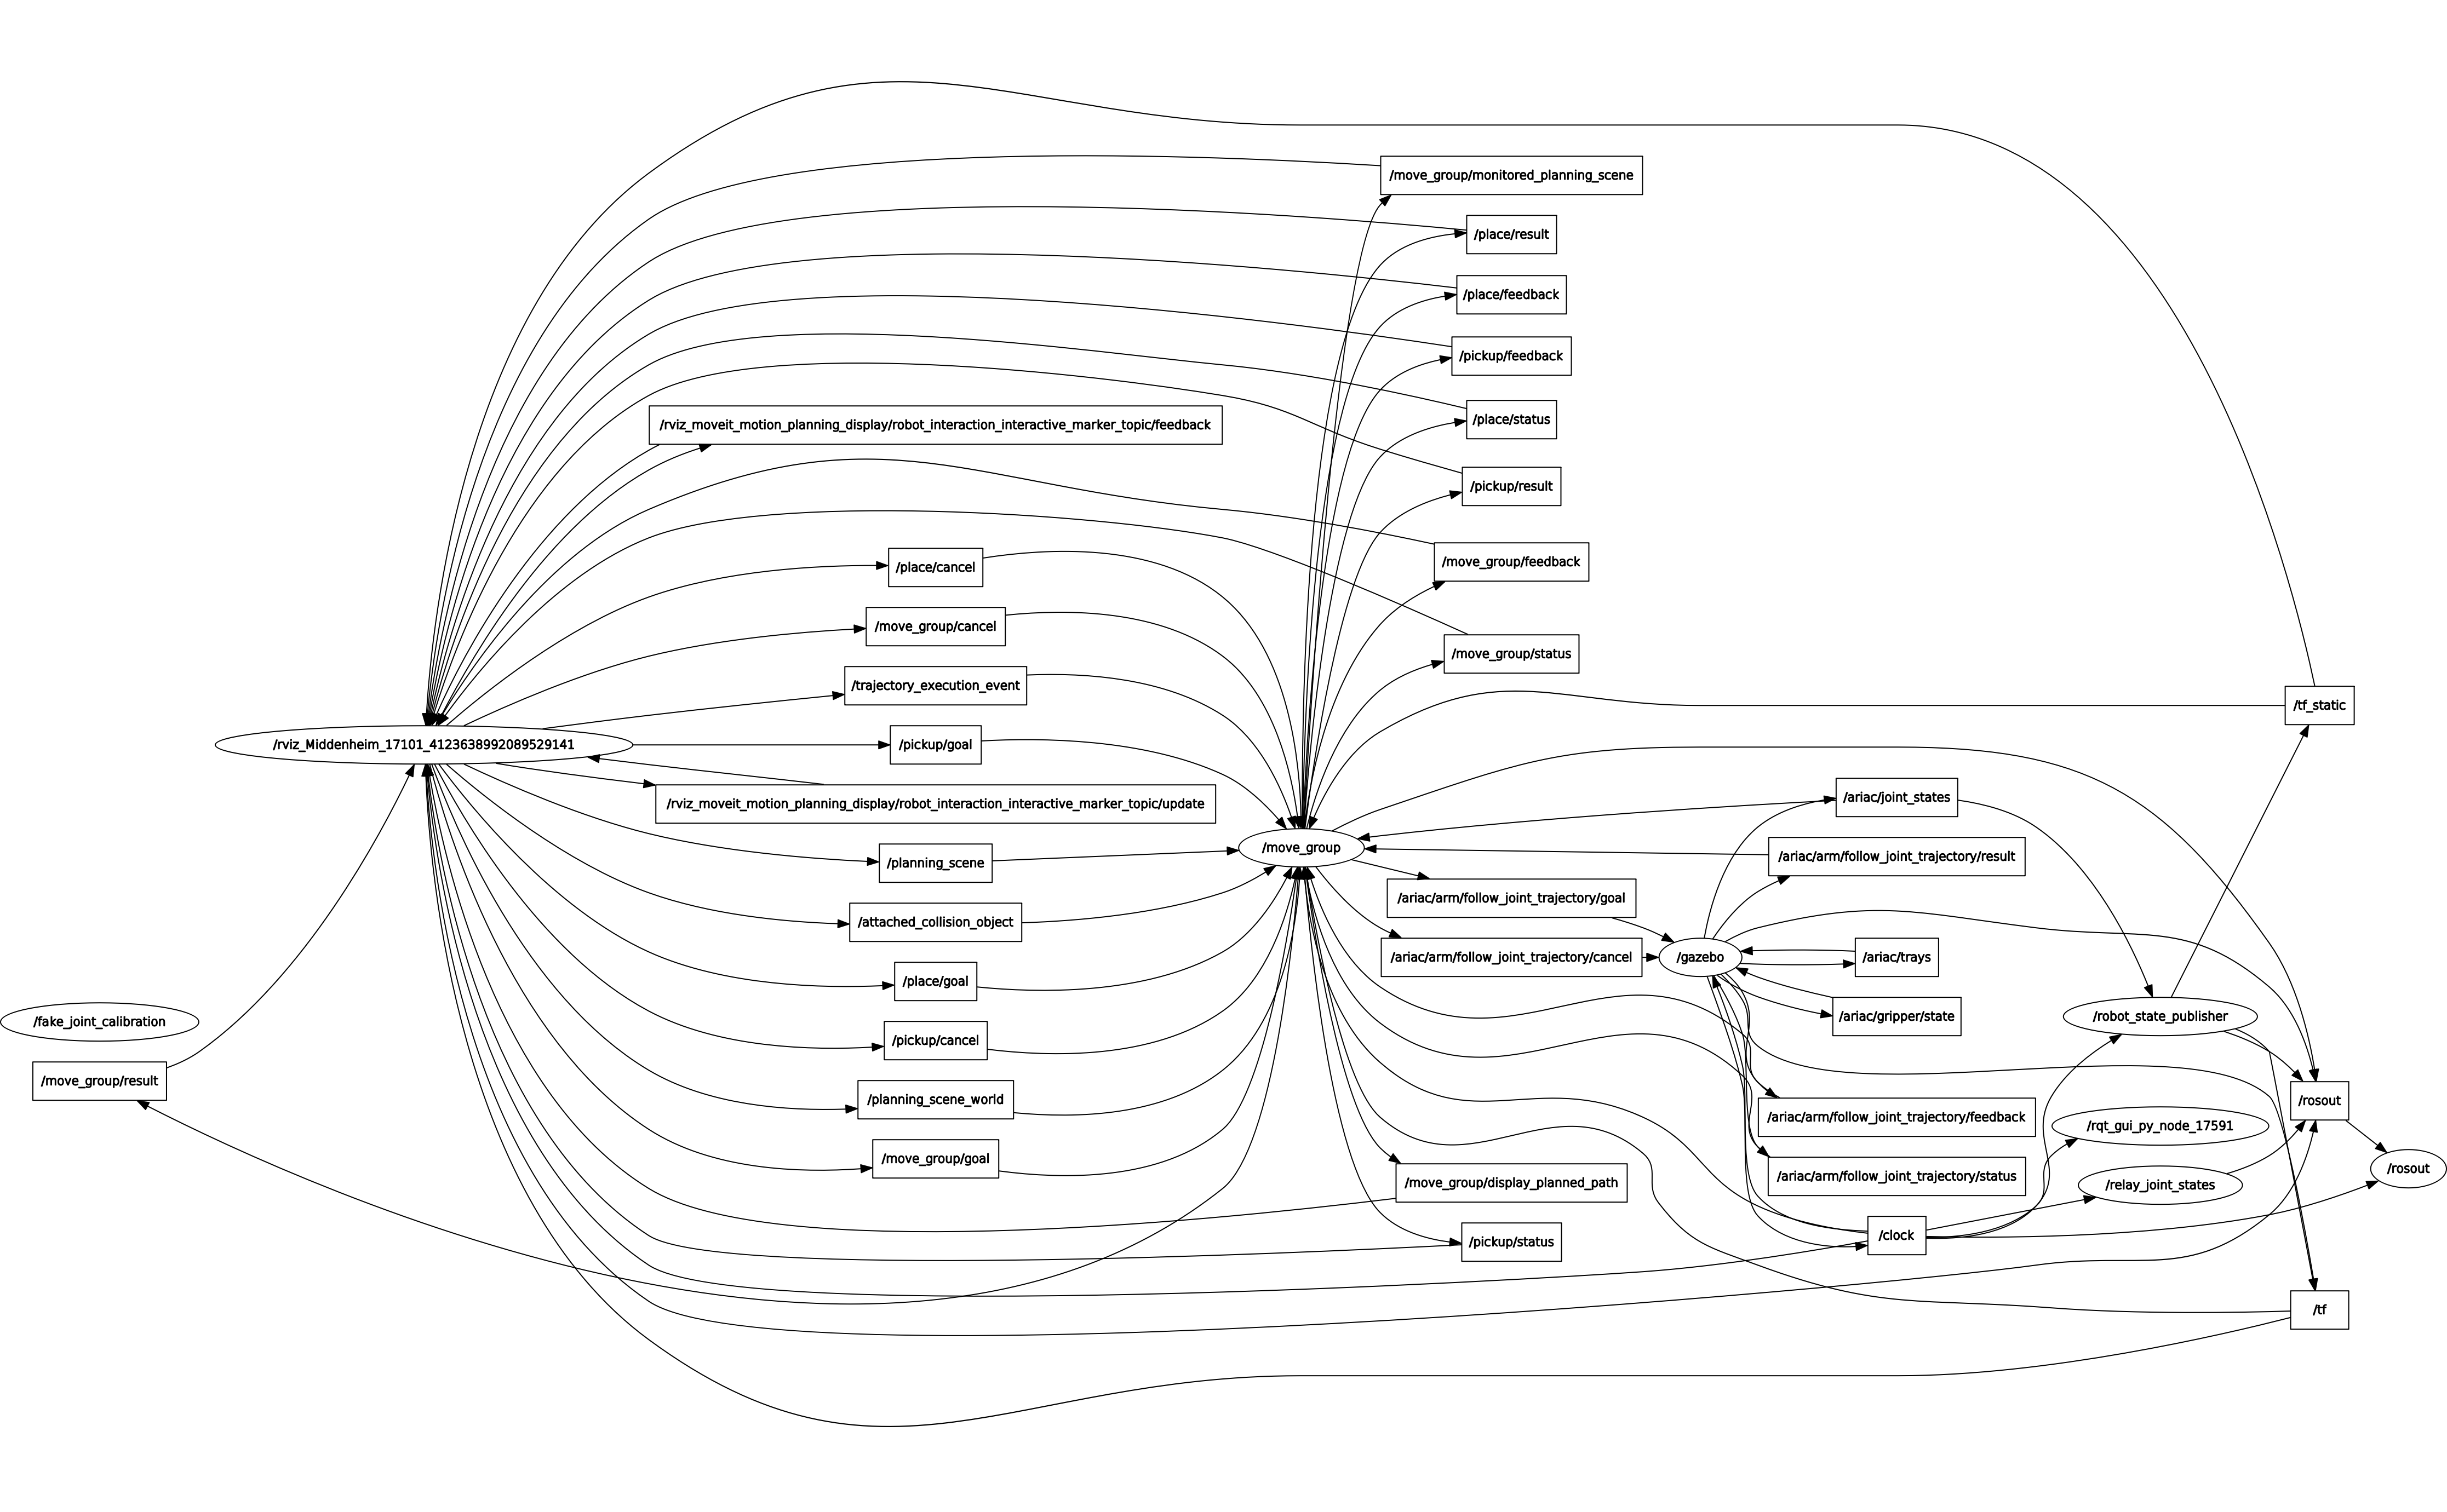
\includegraphics[width=1\textwidth]{moveitgraph01.png}
	\caption{Grafo con la relación de nodos y topic de ARIAC, el brazo, MoveIt y rViz.} \label{fig:moveitgraph1}
\end{figure}

Como se puede apreciar es inmensamente grande, así que usamos las opciones de \textit{rqt} para agrupar nodos y topics e intentar reducir su extensión, obteniendo la imagen de la figura \ref{fig:moveitgraph2}. Sigue siendo un esquema enorme, lo cual nos da una idea de la complejidad de esta herramienta.

\begin{figure}[h]
	\centering
	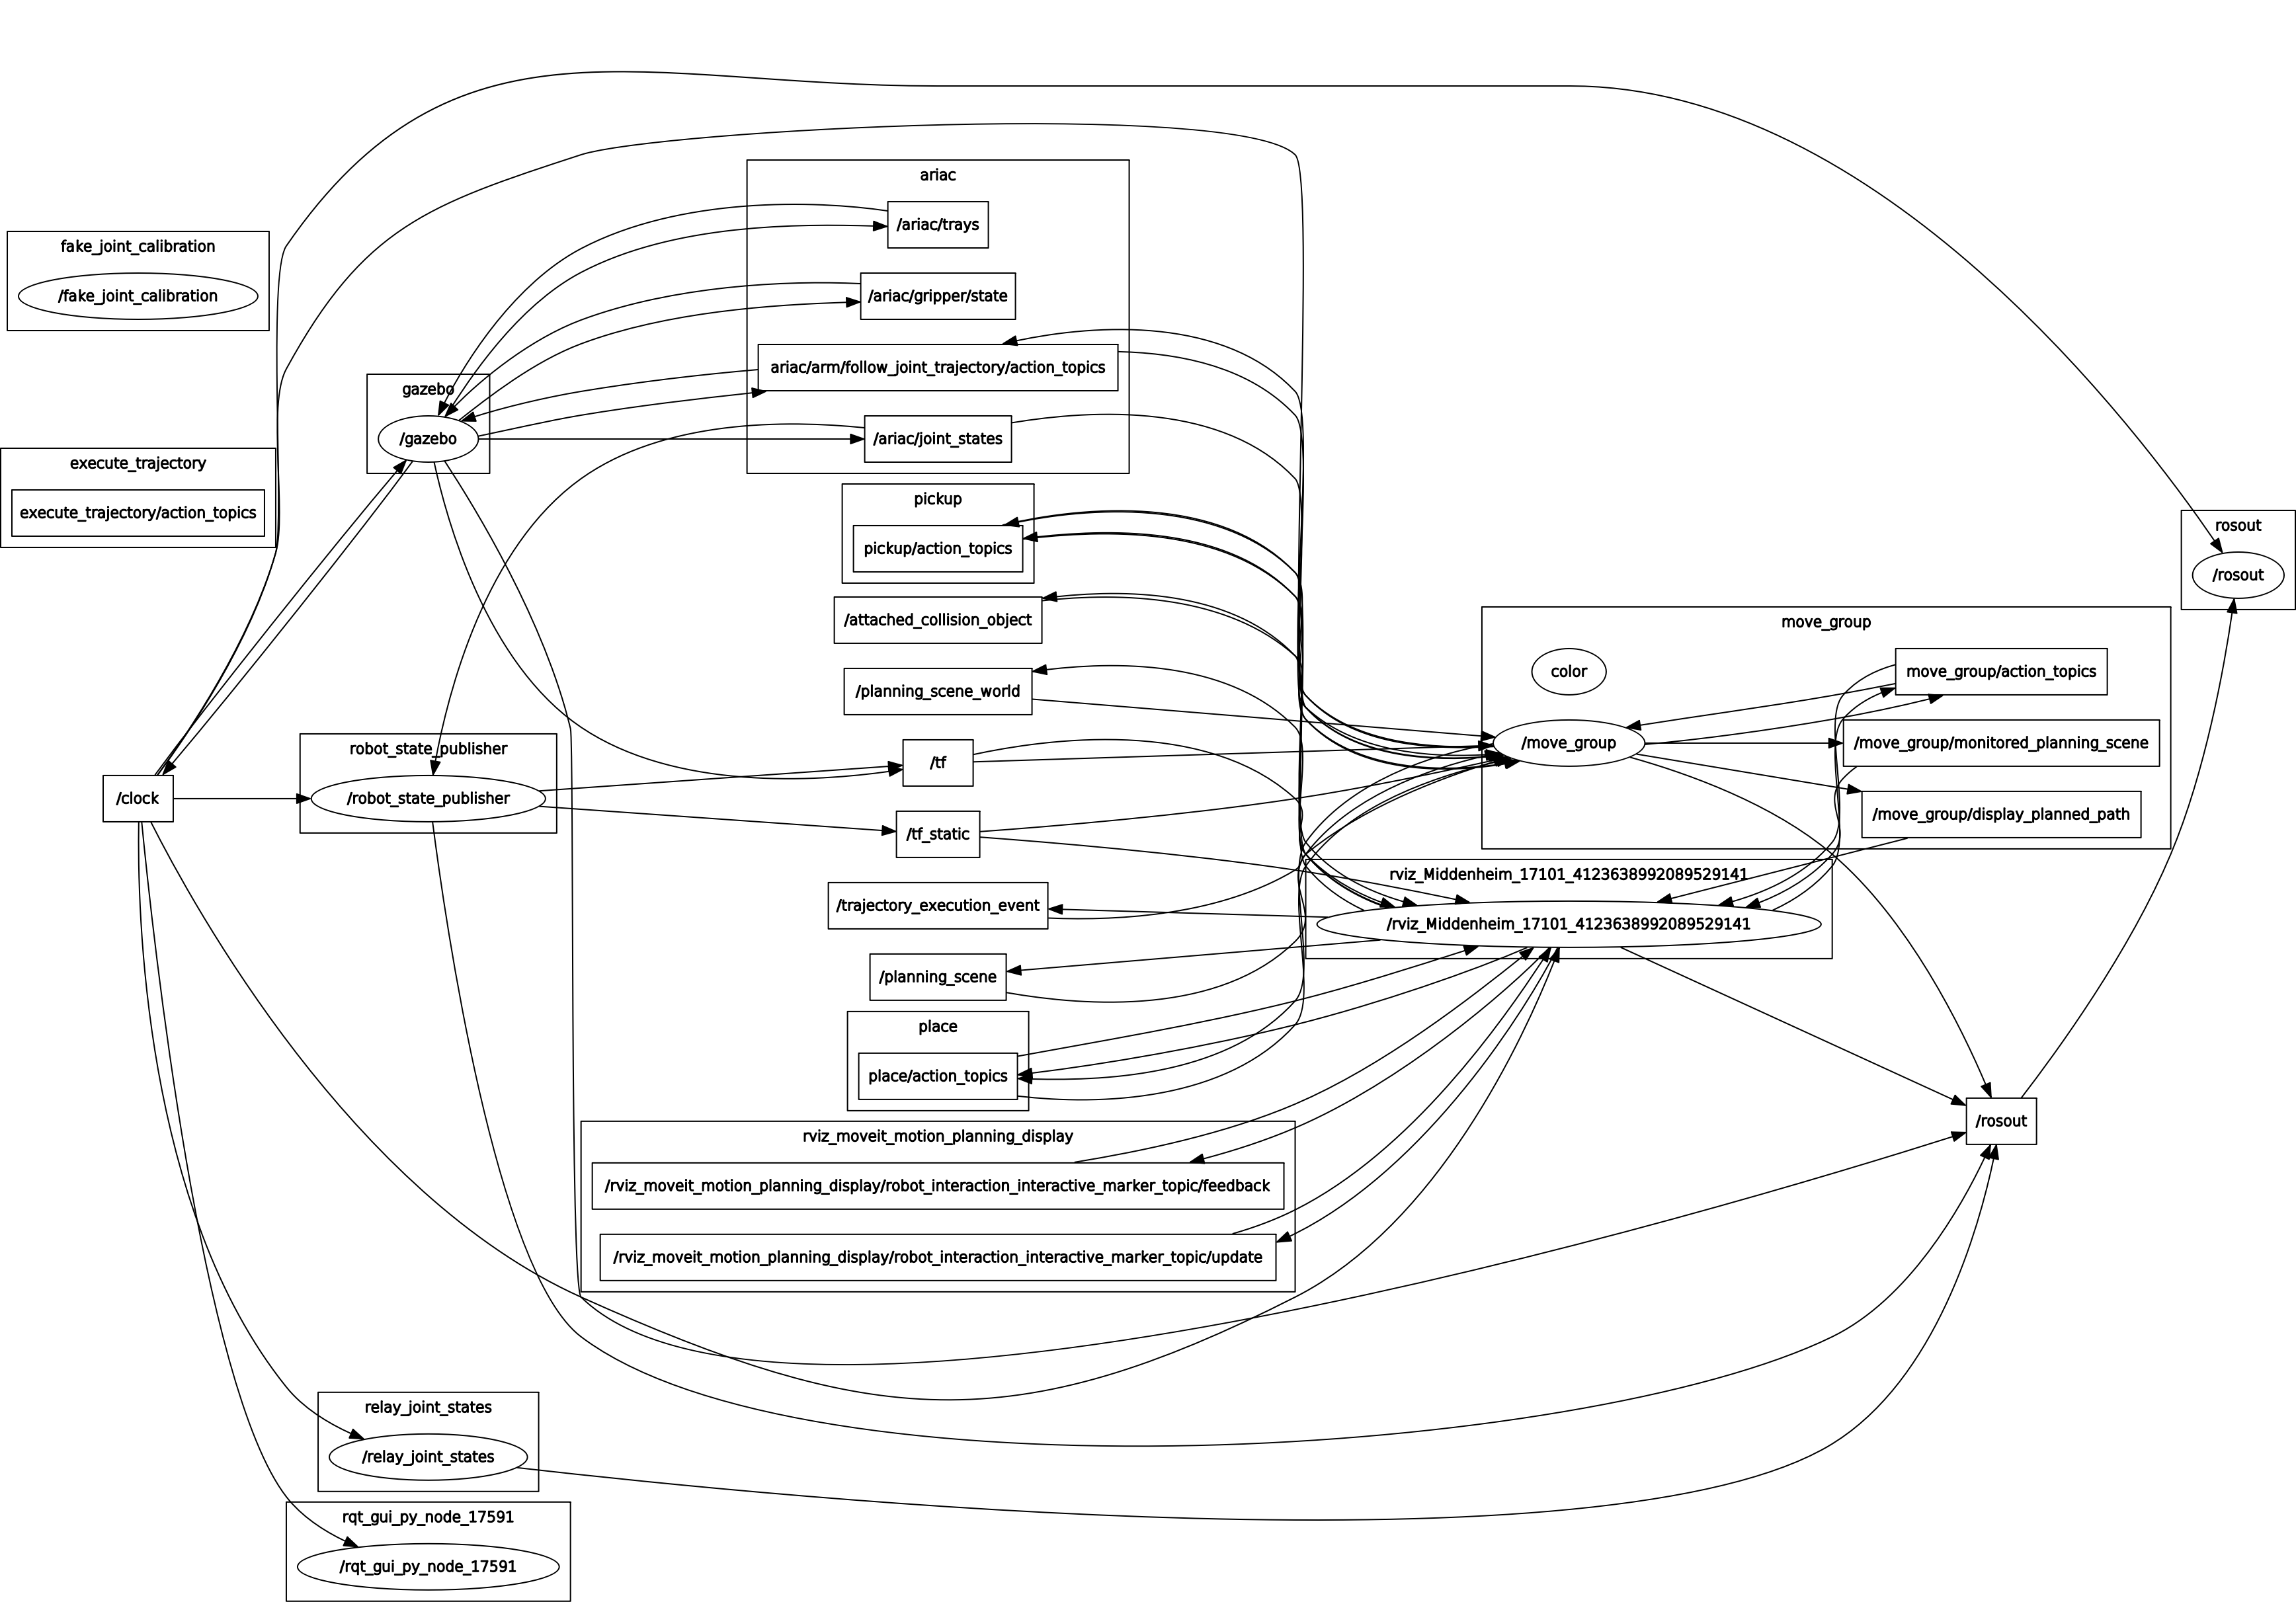
\includegraphics[width=1\textwidth]{moveitgraph02.png}
	\caption{Grafo “simplificado” con la relación de nodos y topic de ARIAC, el brazo, MoveIt y rViz.} \label{fig:moveitgraph2}
\end{figure}

Si acudimos a la documentación oficial nos encontramos con una página\footnote{\url{http://wiki.ros.org/moveit_msgs}} que muestra cómo interactuar con MoveIt. Es una interfaz muy detallada compuesta por mensajes, servicios y acciones de ROS. En la figura \ref{fig:moveitmsgs} se muestra una captura de pantalla de dicha página, con todos los elementos de la interfaz. Como podemos ver es una cantidad enorme de mensajes, cada uno con su propio tipo de estructura, que hace muy complejo y largo trabajar con esta herramienta.

A pesar del atractivo de esta herramienta y de sus posibilidades académicas descartamos seguir investigando en esta dirección, ya que consideramos que es una herramienta que debería de utilizarse una vez que las prácticas con el brazo robótico estén más maduras y permitan una mayor interacción con el alumno.

\begin{figure}[h]
	\centering
	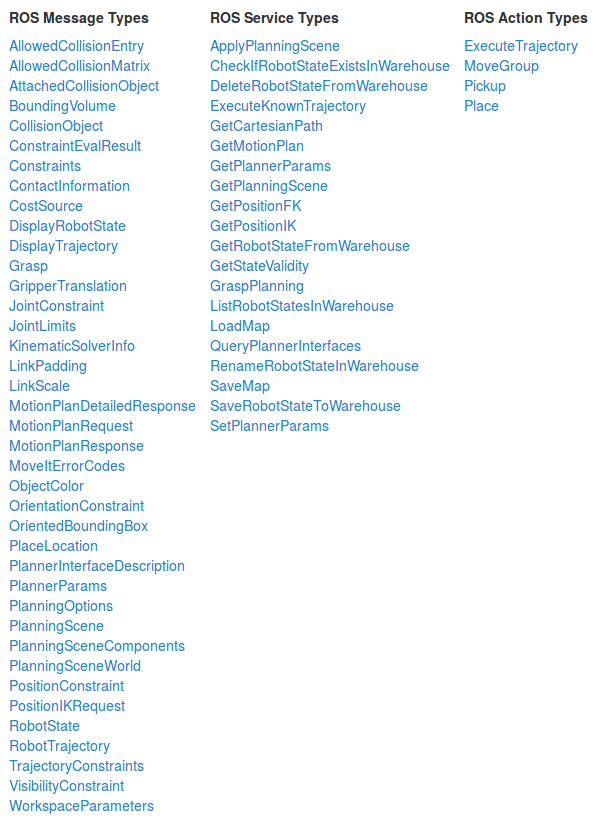
\includegraphics[width=0.85\textwidth]{moveitmsgs.png}
	\caption{Lista de mensajes, servicios y acciones que componen la interfaz de MoveIt.} \label{fig:moveitmsgs}
\end{figure}






